\subsection{Muon Fake Rate}

We summarize the muon fake rate measurements in this appendix section. We use the same
fakeable object definition described in reference \cite{HWW2011}. Also an analogous trigger
selection is used.

\subsubsection{Muon Fake Rate Results}

The muon fake rates measured for the full 2011 data requiring the leading jet $p_{T}$ to be 
larger than $15$ GeV are shown in Figure \ref{fig:mu_fr_Full2011} as a function of the $p_{T}$ 
and $\eta$ of the muon. The fake rates are tabulated in the 
$p_{T}$ and $\eta$ bins used to perform the background estimate in Table \ref{tab:mu_fr_Full2011}.


\begin{figure}[!htbp]
\begin{center}
\subfigure[$p_{T}$]{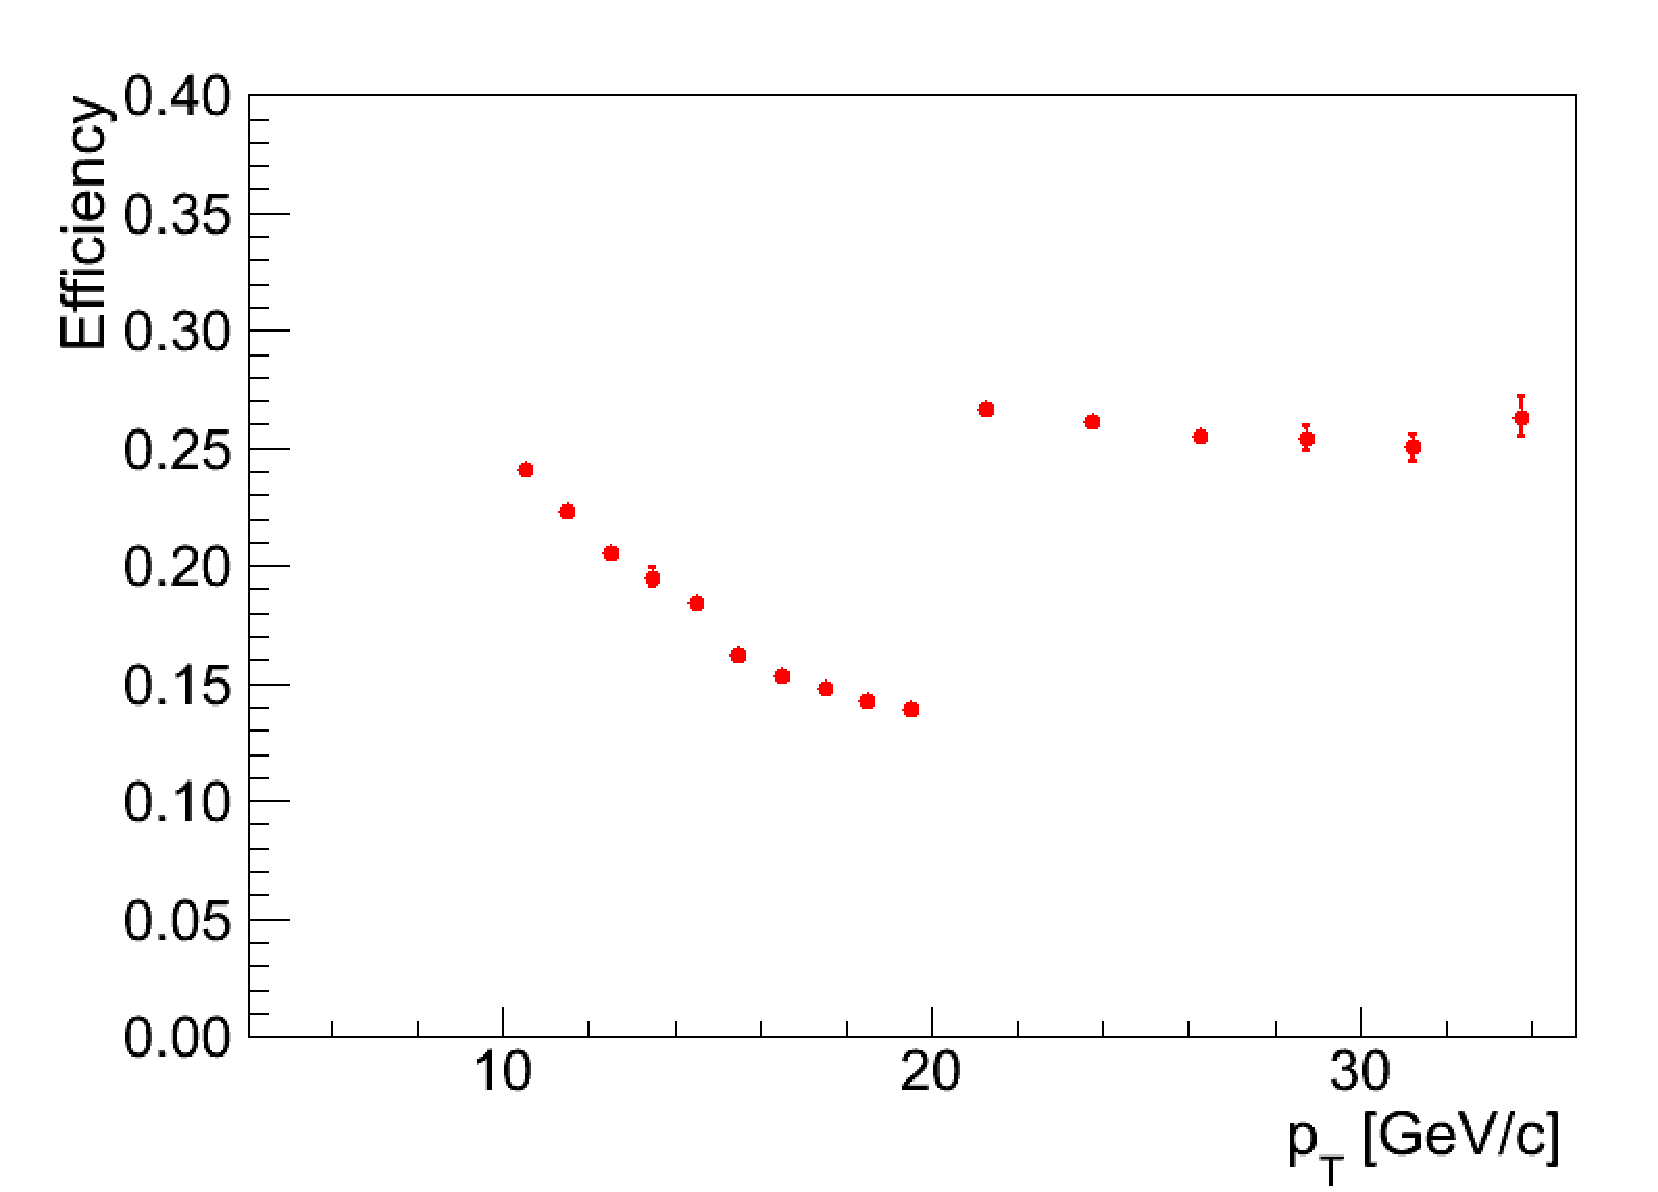
\includegraphics[width=0.45\textwidth]{figures/MuonFakeRate_Pt.pdf}}
\subfigure[$\eta$]{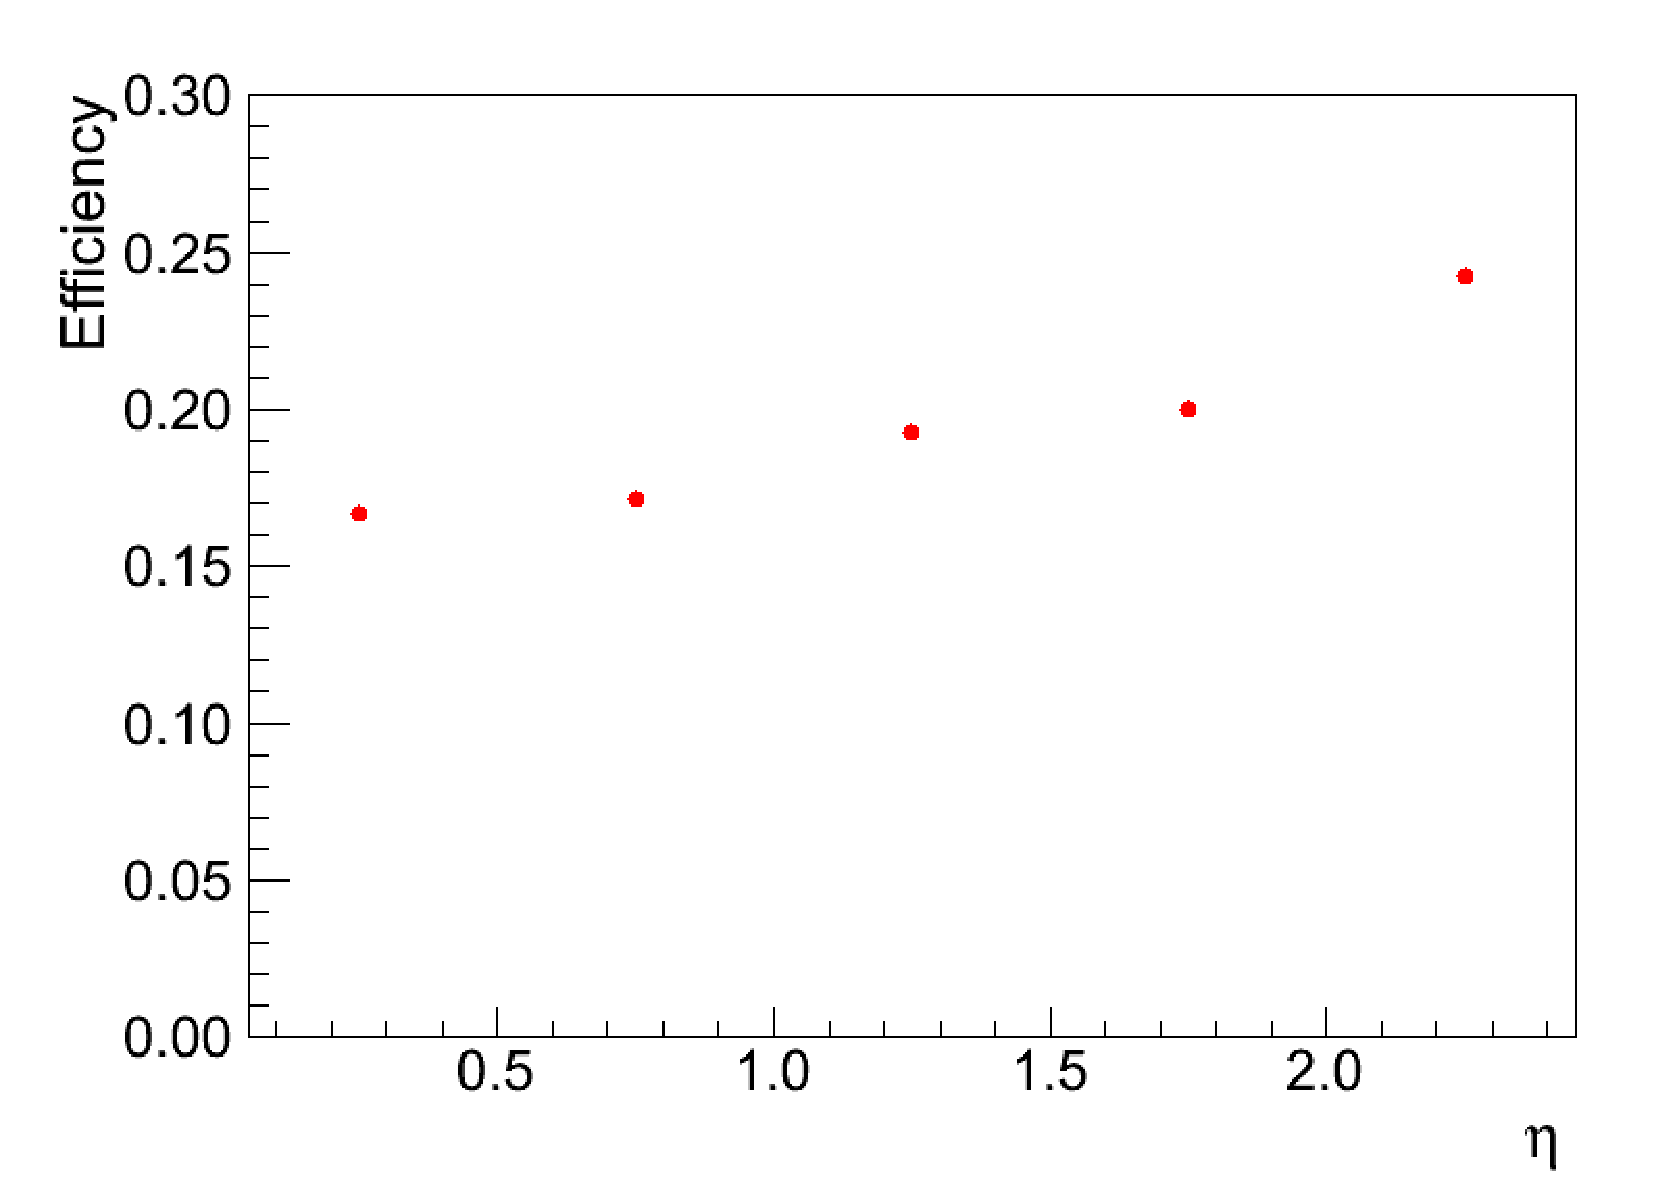
\includegraphics[width=0.45\textwidth]{figures/MuonFakeRate_Eta.pdf}}
\caption{Muon fake rates as a function for $p_{T}$ and $\eta$ for the full 2011 dataset.}
\label{fig:mu_fr_Full2011}
\end{center}
\end{figure}


\begin{table}[!htbp]
\begin{center}
\begin{tabular}{|c|c|c|c|c|c|}

\hline
                       &        $0<\eta<1.0$      &        $1.0<\eta<1.479$  &        $1.479<\eta<2.0$  &        $2.0<\eta<2.5$     \\
\hline
    $10 < p_{T} <= 15$ &        $0.197 +/- 0.002$ &        $0.212 +/- 0.003$ &        $0.230 +/- 0.003$ &        $0.267 +/- 0.004$  \\ 
 \hline
    $15 < p_{T} <= 20$ &        $0.137 +/- 0.001$ &        $0.156 +/- 0.001$ &        $0.172 +/- 0.001$ &        $0.209 +/- 0.003$  \\ 
 \hline
    $20 < p_{T} <= 25$ &        $0.254 +/- 0.002$ &        $0.289 +/- 0.003$ &        $0.254 +/- 0.003$ &        $0.309 +/- 0.006$  \\ 
 \hline
    $25 < p_{T} <= 30$ &        $0.240 +/- 0.004$ &        $0.275 +/- 0.006$ &        $0.253 +/- 0.006$ &        $0.298 +/- 0.011$  \\ 
 \hline
    $30 < p_{T} <= 35$ &        $0.237 +/- 0.006$ &        $0.271 +/- 0.010$ &        $0.257 +/- 0.010$ &        $0.328 +/- 0.021$  \\ 
 \hline

\end{tabular}
\caption{Muon fake rate in $\eta$-$p_T$ using the full 2011 data.
Uncertainties are statistical only. A combination of the {\bf Mu8}, {\bf Mu15}, and {\bf kHLT\_Mu8\_Jet40}
triggers are used, with a $p_{T}$ threshold on the leading jet in the event of $15$ GeV. }
\label{tab:mu_fr_Full2011}
\end{center}
\end{table}


\subsubsection{Pileup Dependence}

Due to the effect of energy from pileup interactions on the electron isolation, there can be a small 
dependence of the fake rate on the number of reconstructed primary vertices. From
Figure \ref{fig:mu_fr_PileupDependence} we observe that the pileup dependence is 
negligible.


\begin{figure}[!htbp]
\begin{center}
\subfigure[Number of Reconstructed Primary Vertices]{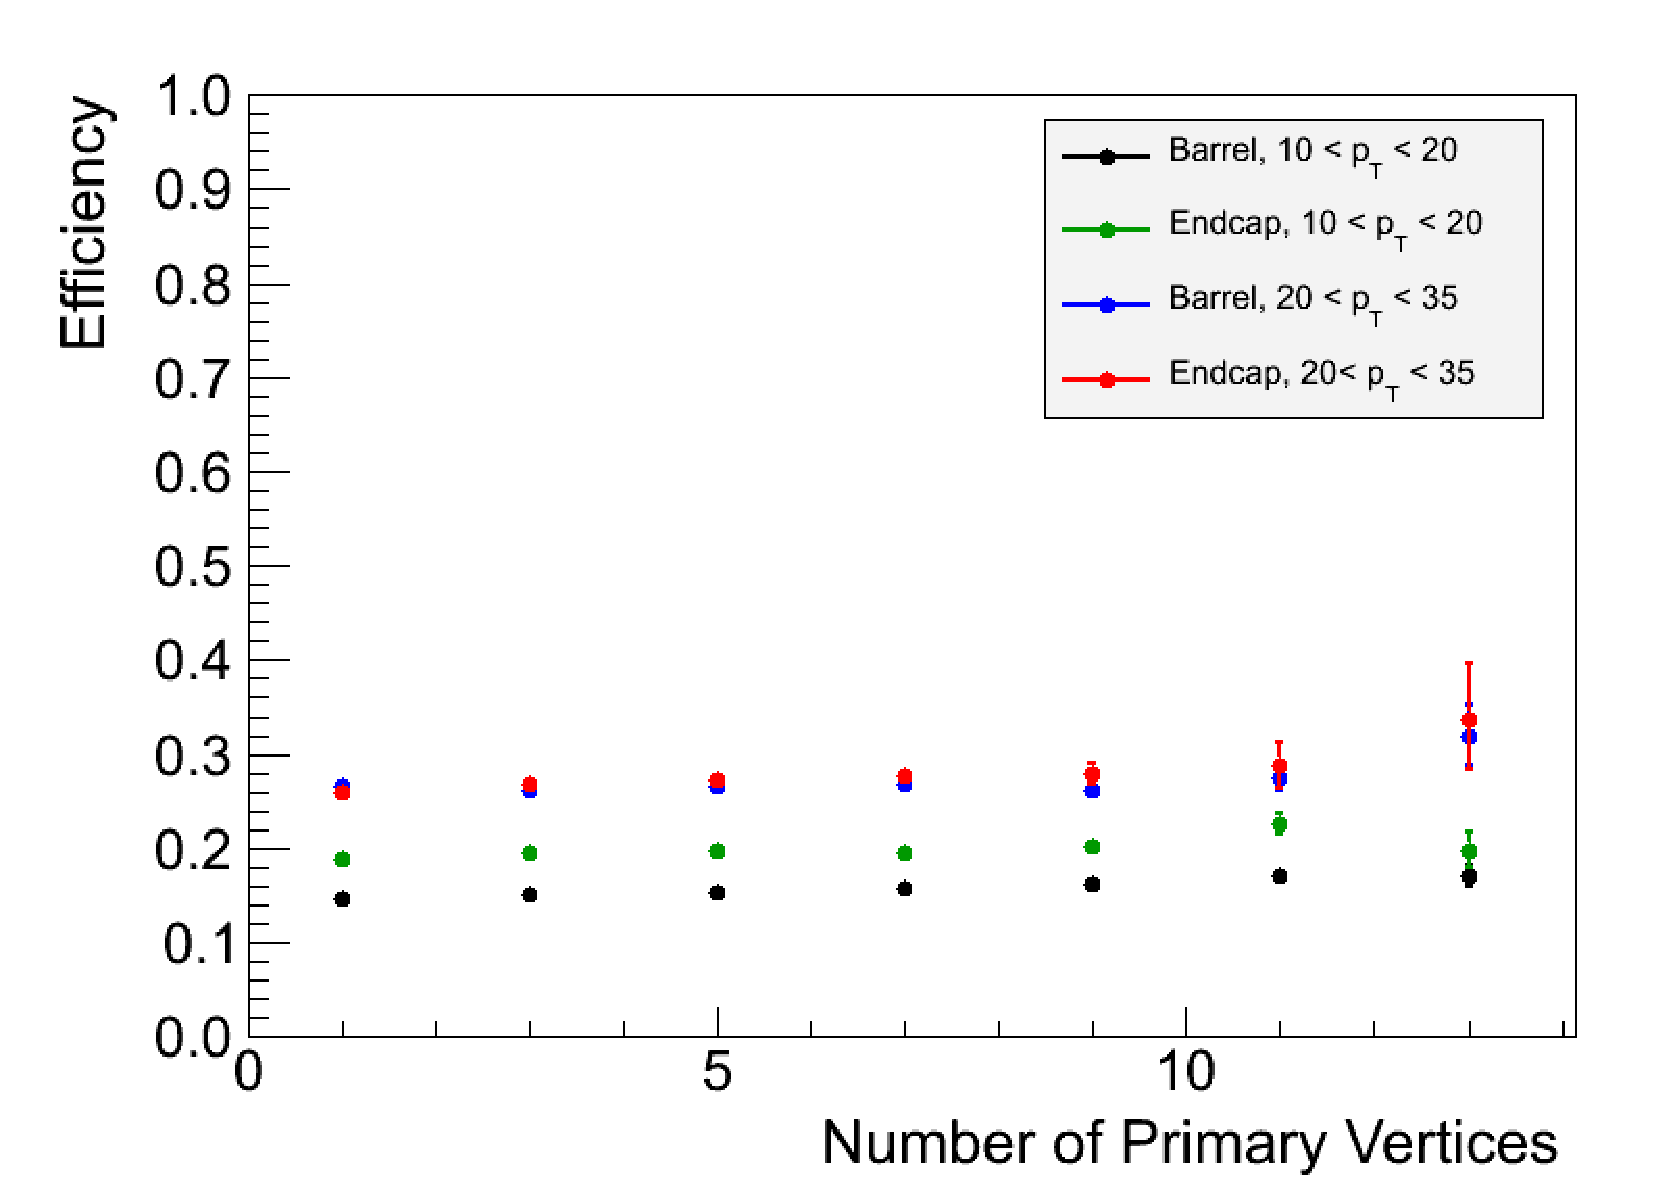
\includegraphics[width=0.45\textwidth]{figures/MuonFakeRate_NVtx.pdf}}
\subfigure[Pileup Energy Density ($\rho$)]{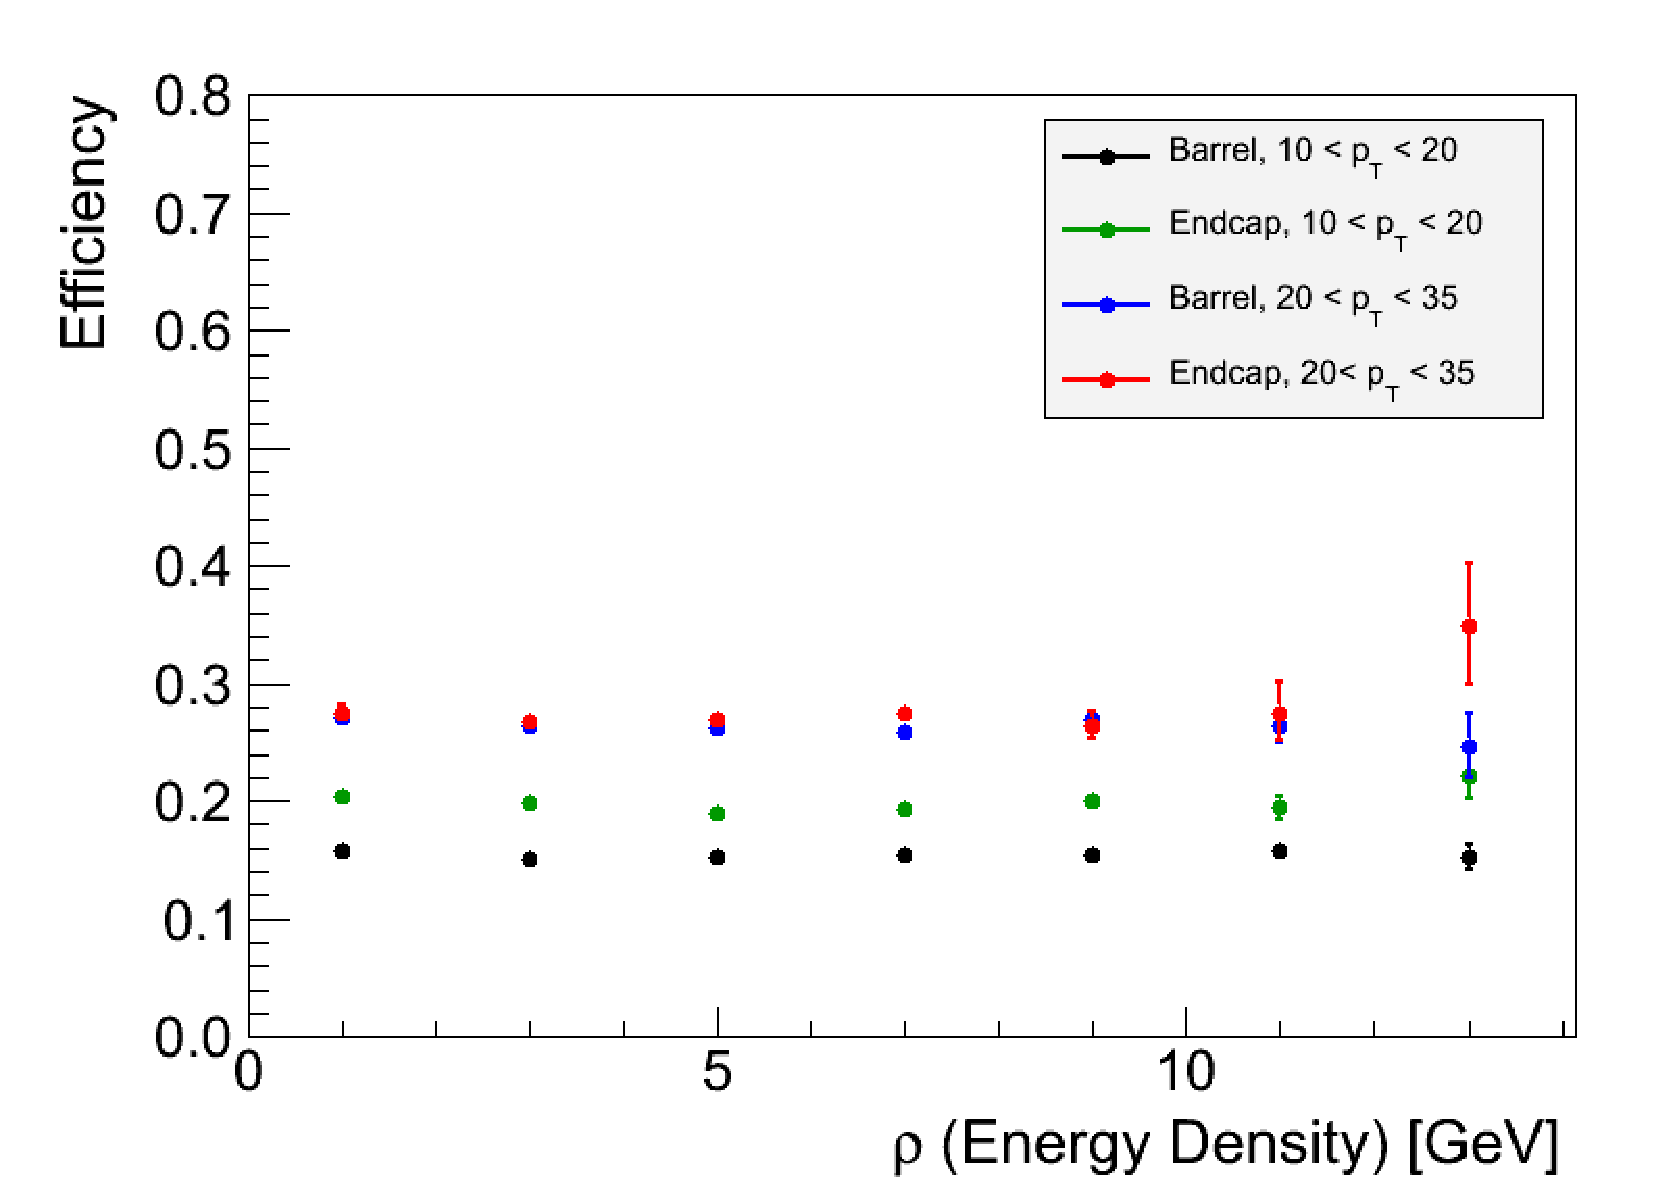
\includegraphics[width=0.45\textwidth]{figures/MuonFakeRate_Rho.pdf}}
\caption{Muon fake rates as a function of the number of reconstructed primary vertices (a) 
and the pileup energy density (b) in four different $p_{T}$ and $\eta$ bins.}
\label{fig:mu_fr_PileupDependence}
\end{center}
\end{figure}  



